%%%%%%%%%%%%%%%%%%%%%%%%%%%%%%%%%%%%%%%%%%%%%%%%%%%%%%%%%%%%%%%%%%%%%%%%%%%%%%%%%%%%%%%
%%%%%%%%%%%%%%%%%%%%%%%%%%%%%%%%%%%%%%%%%%%%%%%%%%%%%%%%%%%%%%%%%%%%%%%%%%%%%%%%%%%%%%%
%%%%%%%%%%%%%%%%%%%%%%%%%%%%%%%%%%%%%%%%%%%%%%%%%%%%%%%%%%%%%%%%%%%%%%%%%%%%%%%%%%%%%%%
\section{Minimização de $||h(x)-a||^2+\alpha ||x-x_{last}||^2$}

%\index{Problema inverso!Não linear}
\index{Minimização do erro quadrático!Não linear}%!Função $||h(x)-a||^2+\alpha ||x-x_{last}||^2$}

\begin{theorem}[Solução iterativa]\label{theo:minhxhxxoxo}
Dados,
um escalar $\alpha \in \mathbb{R}_+$, 
um escalar $x \in \mathbb{R}$, 
um escalar $a \in \mathbb{R}$,  
uma função $h:\mathbb{R} \rightarrow \mathbb{R}$, e 
definida a Eq. (\ref{eq:minhxhxxoxo1}),
\begin{equation}\label{eq:minhxhxxoxo1}
e(x)=||h(x)-a||^2+\alpha ||x-x_{last}||^2,
\end{equation}
considerando que $x_{last}$ é uma constante equivalente a $x_{k-1}$
numa busca iterativa ou equivalente a $p$, 
se decidimos usar uma aproximação linear ao redor de $p$ em $h(x)$; 
é dizer, o segundo somando na Eq. (\ref{eq:minhxhxxoxo1}) 
procura minimizar $||x_{k}-x_{k-1}||^2$.

Se desejamos ter o valor $x=\hat{x}$ que minimiza o escalar $e(x)$,
este valor pode ser achado\footnote{A 
demostração da Eq (\ref{eq:minhxhxxoxo2}) pode ser vista na Prova \ref{proof:theo:minhxhxaxoxo}.} 
 usando iterativamente a Eq. (\ref{eq:minhxhxxoxo2}),
onde  $h'(x)\equiv \frac{d h(x)}{d x}$,
\begin{equation}\label{eq:minhxhxxoxo2}
x_{k+1} \leftarrow x_k+
\frac{ h'(x_k) \left[a-h(x_k)\right] }{\left[h'(x_k)\right]^2+\alpha},
\end{equation}
sendo que em cada iteração se tenta minimizar
\begin{equation}\label{eq:minhxhxxoxo2:ex}
e_{k-1}(x)  \equiv ||h(x)-a||^2 + \alpha||x-x_{k-1}||^2.
\end{equation}
Assim, $\hat{x}$ pode ser achado iniciando a Eq. (\ref{eq:minhxhxxoxo2}) desde um 
$x_{0}$ qualquer, realizando cálculos $x_{k}$ iterativamente, 
ate que $x_{k}$ seja muito próximo a $x_{k-1}$ (convergência de $x_{k}$),
onde pode ser declarado que $\hat{x} \approx x_{k}$.

\textbf{Considerações:}
\begin{itemize}
\item É interessante verificar sempre na Eq. (\ref{eq:minhxhxxoxo2}) 
se  $h'(x_{k-1}) = 0$,
pois indica que existe um ponto de inflexão 
(máximo, mínimo ou ponto de sela) em $e(x_{k-1})$;
consequentemente poderíamos ter achado um mínimo.
\end{itemize}

\end{theorem}

\begin{tcbattention}
\begin{itemize}
\item O Teorema \ref{theo:minhxhxxoxo} pode ser usado para achar um ponto $x$
que minimize as funções de custo $||h(x)-a||^2$ e
 $||x_{k}-x_{k-1}||^2$ de forma simultânea, ponderando estas seguindo o fator $\alpha$.
\item No Teorema \ref{theo:minhxhxxoxo} o valor $x=\hat{x}$ 
que minimiza $e(x)$ não necessariamente minimiza $||h(x)-a||^2$.
\end{itemize}
\end{tcbattention}
%%%%%%%%%%%%%%%%%%%%%%%%%%%%%%%%%%%%%%%%%%%%%%%%%%%%%%%%%%%%%%%%%%%%%%%%%%%%%%%%
\subsection{Exemplos de minimização de $||h(x)-a||^2+\alpha ||x-x_{last}||^2$}


\begin{example}\label{ex:minhxhxxoxo1}
Conhecida uma função $h(x)=x^2(x^2-1)$, o valor $a=1$ do contradomínio de $h(x)$,
e o fator $\alpha=1.2$,
achar o valor $\hat{x}$ que minimize $e(x)=||h(x)-a||^2+\alpha||x-x_{last}||^2$.
\end{example}
\begin{SolutionT}[Relativa ao Exemplo \ref{ex:minhxhxxoxo1}:]\label{sol:minhxhxxoxo1}
 A Fig. \ref{fig:hxccasesa} nos mostra o processo de busca de um mínimo
 de $e(x)$. A busca inicia em $x_0=-1.4$,
 todos os valores $x_{k}$ podem ser vistos na Tabela \ref{tab:hxccases1}. 
Neste caso a busca iterativa indicada pela Eq. (\ref{eq:minhxhxxoxo2}) converge sem problemas 
em $\hat{x}\approx x_3 =-1.2721$ com $e(x_3)=8.7404e-08$.

É interesante lembrar que os valores $x_{min}=\pm \sqrt{\frac{1+\sqrt{5}}{2}}$ 
$\approx \pm 1.27202$ provocam $h(x_{min})=a$.
\end{SolutionT}

\begin{table}[!h]
\centering
\begin{tabular}{|l|l|l|l|l|}
\hline
$k$      & 0 & 1 & 2 & 3 \\ \hline
$x_k$    & -1.4000 & -1.2941 & -1.2734 & -1.2721 \\ \hline
$e_k(x_k)$ & 7.7722e-01 & 1.6835e-02 & 6.2390e-05 & 8.7404e-08 \\ \hline
\end{tabular}
\caption{Resposta iterativa do Exemplo \ref{ex:minhxhxxoxo1}.}
\label{tab:hxccases1}
\end{table}

\begin{figure}[!h]
    \centering
    \begin{subfigure}[b]{0.49\textwidth}
        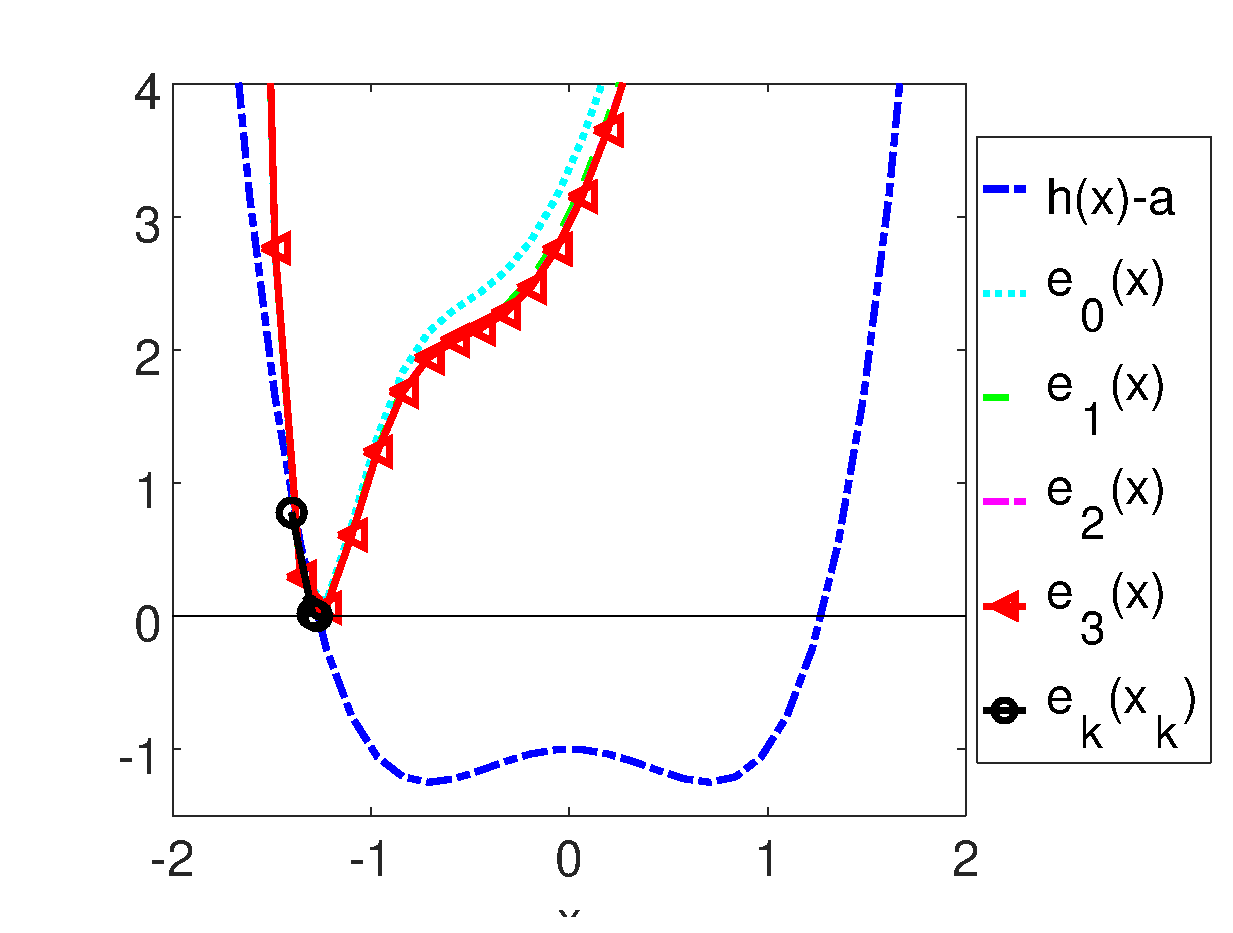
\includegraphics[width=\textwidth]{chapters/minimization-hx/mfiles/hx_a_alphax_last/minimizando_hx_a_alphax_1.eps}
        \caption{Usando $h(x)=x^2(x^2-1)$, $a=1$ e $\alpha=1.2$, quando as iterações convergem.}
        \label{fig:hxccasesa}
    \end{subfigure}
    ~ %add desired spacing between images, e. g. ~, \quad, \qquad, \hfill etc. 
      %(or a blank line to force the subfigure onto a new line)
    \begin{subfigure}[b]{0.49\textwidth}
        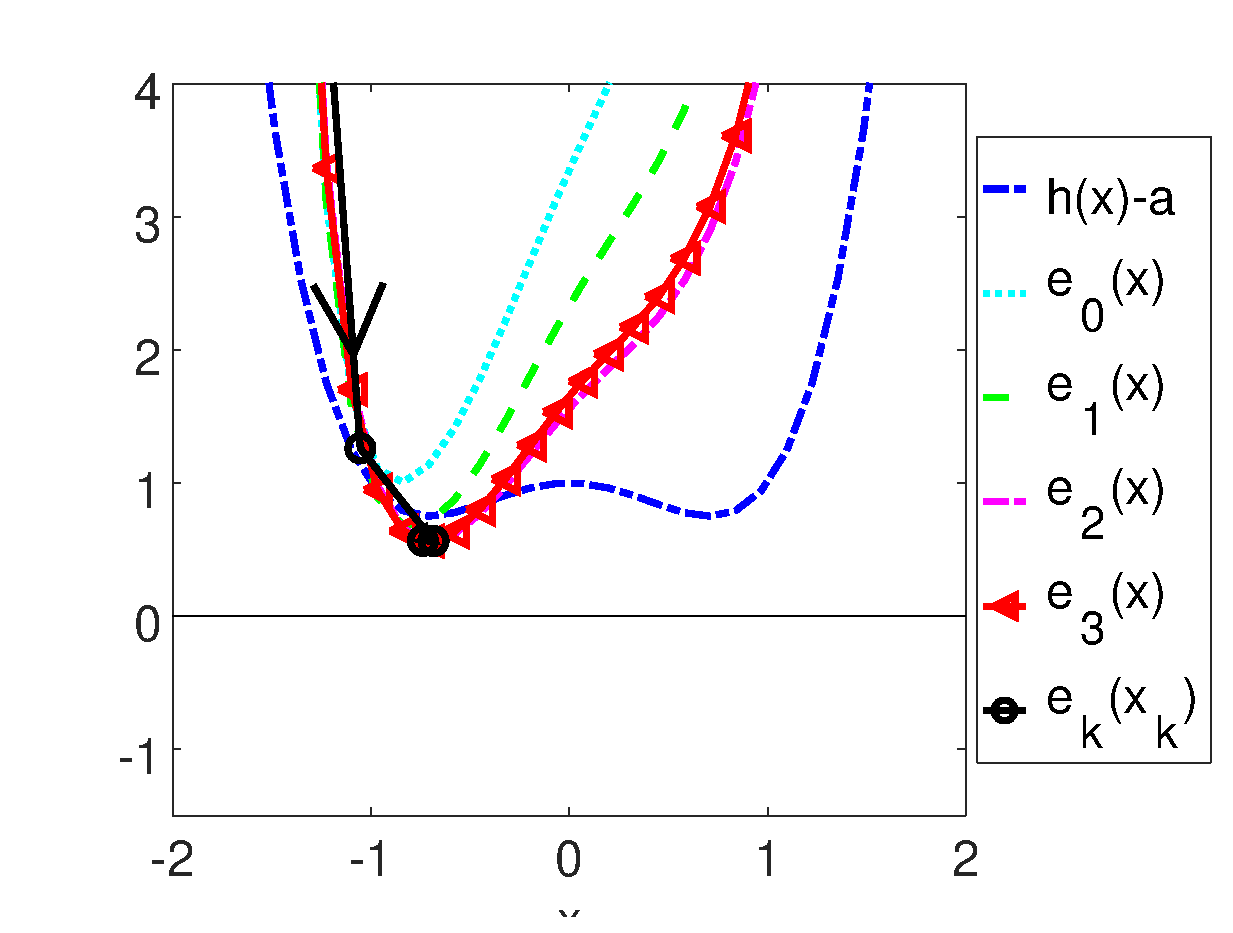
\includegraphics[width=\textwidth]{chapters/minimization-hx/mfiles/hx_a_alphax_last/minimizando_hx_a_alphax_2.eps}
        \caption{Usando $h(x)=x^2(x^2-1)$, $a=-1$ e $\alpha=1.2$, quando as iterações convergem.}
        \label{fig:hxccasesb}
    \end{subfigure}
    \caption{Comportamento para $h(x)=x^2(x^2-1)$ da equação iterativa do Teorema \ref{ex:minhxhxxoxo1}.}
    \label{fig:hxccases}
\end{figure}

\begin{example}\label{ex:minhxhxxoxo2}
Conhecida uma função $h(x)=x^2(x^2-1)$, o valor $a=-1$ que não existe no contradomínio de $h(x)$,
e o fator $\alpha=1.2$,
achar o valor $\hat{x}$ que minimize $e(x)=||h(x)-a||^2+\alpha||x-x_{last}||^2$.
\end{example}
\begin{SolutionT}[Relativa ao Exemplo \ref{ex:minhxhxxoxo2}:]\label{sol:minhxhxxoxo2}
 A Fig. \ref{fig:hxccasesb} nos mostra o processo de busca de um mínimo
 de $e(x)$. A busca inicia em $x_0=-1.4$,
 todos os valores $x_{k}$ podem ser vistos na Tabela \ref{tab:hxccases2}. 
Neste caso a busca iterativa indicada pela Eq. (\ref{eq:minhxhxxoxo2}) converge sem problemas 
em $\hat{x}\approx x_3 =-0.73819$ com $e(x_3)=0.56553$.
\end{SolutionT}

\begin{table}[!h]
\centering
\begin{tabular}{|l|l|l|l|l|}
\hline
$k$      & 0 & 1 & 2 & 3 \\ \hline
$x_k$    & -1.40000 & -1.05377 & -0.68441 & -0.73819 \\ \hline
$e_k(x_k)$ & 8.30362 &  1.26028 &  0.56400 &  0.56553 \\ \hline
\end{tabular}
\caption{Resposta iterativa do Exemplo \ref{ex:minhxhxxoxo2}.}
\label{tab:hxccases2}
\end{table}

